\chapter{Additional Material for Chapter 4}
\graphicspath{{figures/ch_4/}}
\addtocontents{toc}{\protect\setcounter{tocdepth}{0}}

\section{Simulation study}

We performed a simulation study on 200 datasets to validate our models.
We use the same prior distributions for the parameters as in the main text.
These distributions are presented in Table~\ref{ch_4:table:simulation_parameters}.
We purposely chose parameter values that resulted in data similar to the Orange Country data used in the main text.
Exact values for these parameters are presented in Table~\ref{ch_4:table:simulation_parameters}.
One of the 200 simulated datasets is presented in Figure~\ref{ch_4:fig:simulated_binned_data_plot}.
Figures~\ref{ch_4:fig:single_generated_quantities_simulation_scalar_plot}--\ref{ch_4:fig:single_generated_quantities_simulation_compartment_plot} present the prior and posterior distribution for this single dataset.
Figures~\ref{ch_4:fig:generated_quantities_simulation_scalar_coverage_plot}--\ref{ch_4:fig:generated_quantities_simulation_time_varying_shrinkage_plot} show coverage and contraction properties for the whole simulation study.
Contraction is calculated as one minus the ratio of standard deviation of the posterior and the prior.
Commentary on these results is presented in Section~\ref{ch_4:sec:results} of the main text.

\begin{table}
	\caption[Parameters and priors.]{Model parameters and their prior distributions.}
	\label{ch_4:table:priors}
	\scriptsize\centering
	\begin{tabularx}{\columnwidth}{cXllc}
	\thead{Parameter} & \thead{Interpretation} & \thead{Prior} & \thead{Prior Median\\ (95\% Interval)} & \thead{Source} \\ \hline
$S_0$ & Initial susceptible proportion & Logit-Normal(6, 0.25) & \makecell{0.998 \\ (0.993, 0.999)} & \\
$\tilde{I}_{0}$ & Initial proportion of non-susceptibles who are infectious & Logit-Normal(0.6, 0.0009) & \makecell{0.646 \\ (0.632, 0.659)} & \\
$\exp\left(\tilde{R}_{0,1}\right)$ & Initial basic reproduction number & Log-Normal(0, 0.0625) & \makecell{1.000 \\ (0.613, 1.630)} & \\
$1 / \gamma$ & Mean latent period (weeks) & Log-Normal(-0.25, 0.01) & \makecell{0.779 \\ (0.640, 0.947)} & \cite{Xin2021} \\
$1 / \nu$ & Mean infectious period (weeks) & Log-Normal(0.15, 0.01) & \makecell{1.160 \\ (0.955, 1.410)} & \cite{Byrnee039856} \\
$\expit\left(\tilde{\eta}_1\right)$ & Initial infection fatality ratio & Logit-Normal(-5.3, 0.04) & \makecell{0.00497 \\ (0.00336, 0.00733)} & \cite{Bruckner2021} \\
$\rho^D$ & Mean death detection rate & Logit-Normal(2.3, 0.04) & \makecell{0.909 \\ (0.871, 0.937)} & \cite{Bruckner2021} \\
$\phi_D$ & over-dispersion in observed deaths Negative-Binomial model & Log-Normal(4.16, 0.293) & \makecell{ 63.9 \\ ( 22.1, 185.0)} & \\
$\exp\left(\tilde{\alpha}_1\right)$ & Initial proportion in proportional odds test positivity model & Log-Normal(1.35, 0.0121) & \makecell{3.86 \\ (3.11, 4.79)} & \\
$\phi_C$ & over-dispersion in observed cases beta-binomial model & Log-Normal(6.5, 0.0673) & \makecell{ 665 \\ (400, 1110)} & \\
$\sigma_{R_0}$ & Standard deviation of log-Guassian Markov random field for time-varying $R_0$ & Log-Normal(-1.9, 0.09) & \makecell{0.1500 \\ (0.0831, 0.2690)} & \\
$\sigma_\eta$ & Standard deviation of logit-Guassian Markov random field for time-varying $\eta$ & Log-Normal(-2.4, 0.0144) & \makecell{0.0907 \\ (0.0717, 0.1150)} & \\
$\sigma_\alpha$ & Standard deviation of log-Guassian Markov random field for time-varying $\alpha$ & Log-Normal(-2.7, 0.0225) & \makecell{0.0672 \\ (0.0501, 0.0902)} & \\
\hline
$\tilde{\rho}^Y_1$ & Initial case detection rate & Logit-Normal(-2.5, 0.01) & \makecell{0.0759 \\ (0.0632, 0.0908)} & \cite{Bruckner2021} \\
$\phi_Y$ & over-dispersion in observed cases Negative-Binomial model & Log-Normal(3.93, 0.0684) & \makecell{51.1 \\ (30.6, 85.3)} & \\
$\sigma_{\rho^Y}$ & Standard deviation of logit-Guassian Markov random field for time-varying $\rho^Y$ & Log-Normal(-2.2, 0.04) & \makecell{0.1110 \\ (0.0749, 0.1640)} &
	\end{tabularx}
\end{table}

\begin{table}%[htbp]
	\caption[Simulation parameters.]{Simulation parameters.}
	\label{ch_4:table:simulation_parameters}
	\scriptsize\centering
	\begin{tabularx}{\columnwidth}{cXllc}
	\thead{Parameter} & \thead{Interpretation} & \thead{Value}  \\ \hline
$S_0$ & Initial susceptible proportion & 0.9979 \\
$\tilde{I}_{0}$ & Initial proportion of non-susceptibles who are infectious & 0.6455 \\
$\exp\left(\tilde{R}_{0,1}\right)$ & Initial basic reproduction number & 1.2602 \\
$1 / \gamma$ & Mean latent period (weeks) &  0.7697 \\
$1 / \nu$ & Mean infectious period (weeks) & 1.1997 \\
$\expit\left(\tilde{\eta}_1\right)$ & Initial infection fatality ratio & 0.0005 \\
$\rho^D$ & Mean death detection rate &  0.9061 \\
$\phi_D$ & over-dispersion in observed deaths Negative-Binomial model & 87.2776 \\
$\exp\left(\tilde{\alpha}_1\right)$ & Initial proportion in proportional odds test positivity model & 4.3958 \\
$\phi_C$ & over-dispersion in observed cases Beta-Binomial model & 1,026.6765 \\
$\sigma_{R_0}$ & Standard deviation of log-Guassian Markov random field for time-varying $R_0$ & 0.1481 \\
$\sigma_\eta$ & Standard deviation of logit-Guassian Markov random field for time-varying $\eta$ & 0.0944 \\
$\sigma_\alpha$ & Standard deviation of log-Guassian Markov random field for time-varying $\alpha$ & 0.0696 \\
\hline
	\end{tabularx}
\end{table}

\begin{figure}[h]
    \centering
    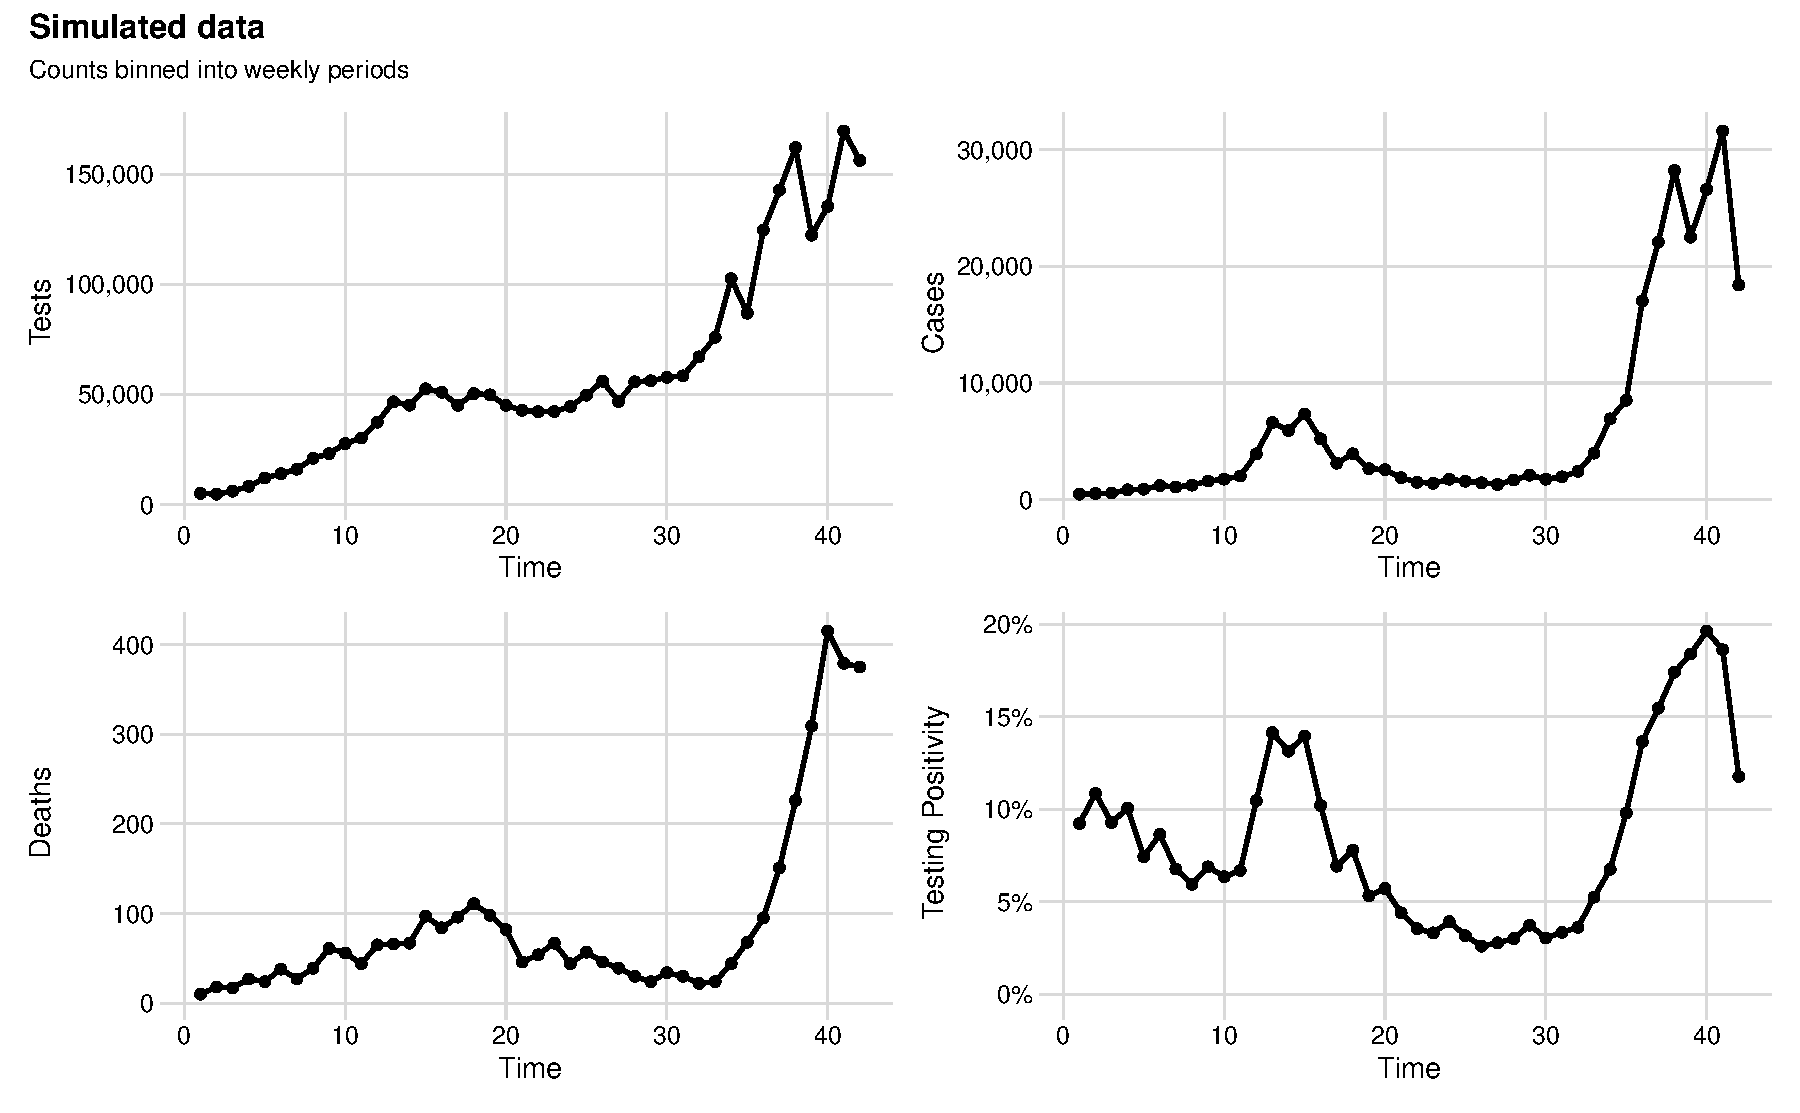
\includegraphics[width=1.0\columnwidth]{simulated_binned_data_plot}
    \caption{
    Simulated data.
    The figure shows weekly counts of tests, cases (positive tests), reported deaths due to COVID-19, as well testing positivity.}
    \label{ch_4:fig:simulated_binned_data_plot}
\end{figure}

\begin{figure}[htbp]
    \centering
    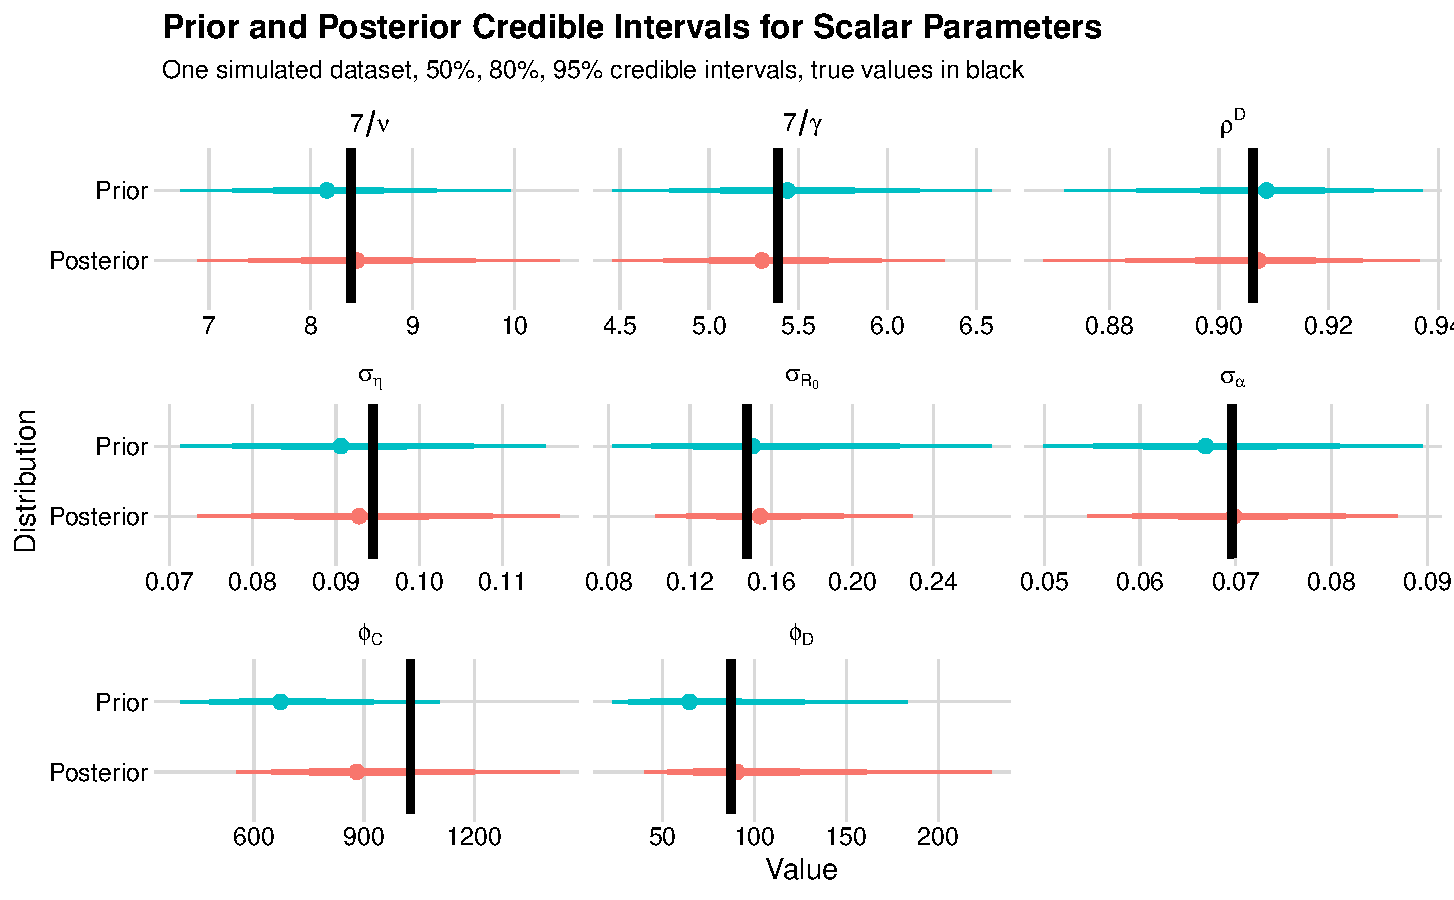
\includegraphics[width=1.0\columnwidth]{single_generated_quantities_simulation_scalar_plot}
    \caption{Prior and posterior credible intervals for scalar parameters for a model fit to the dataset presented in Figure~\ref{ch_4:fig:simulated_binned_data_plot}.
    True values for the simulated parameters are indicated by solid black lines.}
    \label{ch_4:fig:single_generated_quantities_simulation_scalar_plot}
\end{figure}

\begin{figure}[htbp]
    \centering
    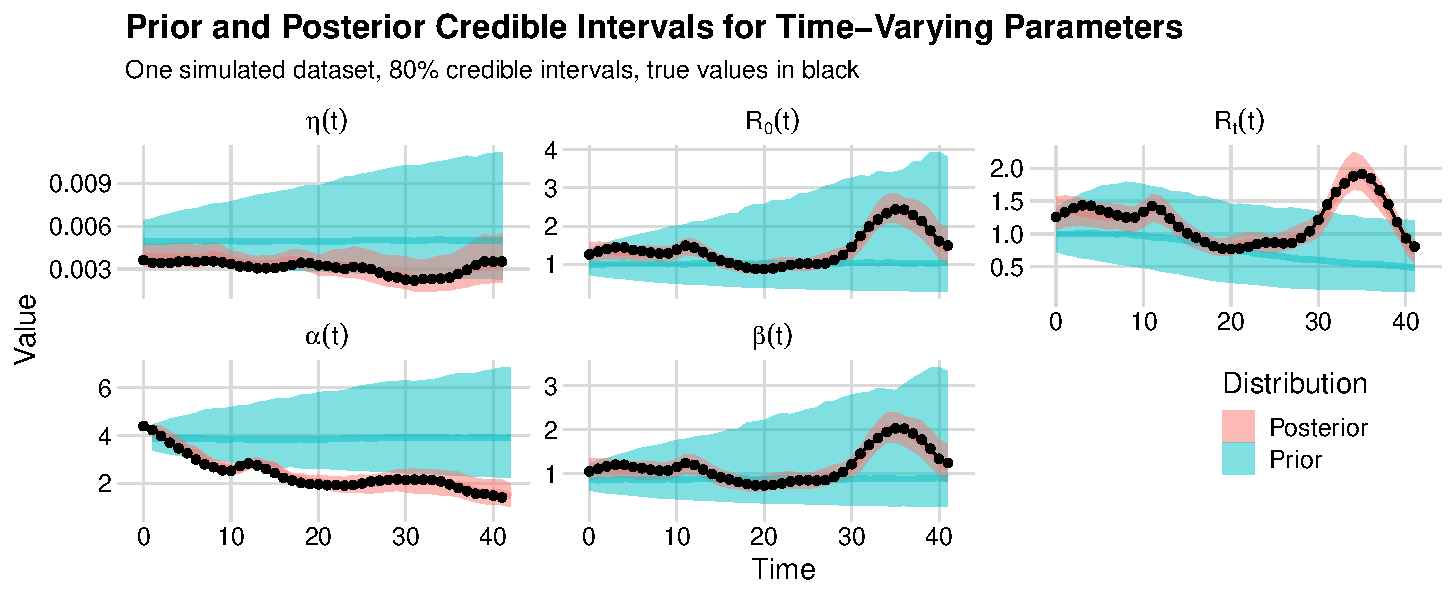
\includegraphics[width=1.0\columnwidth]{single_generated_quantities_simulation_time_varying_plot}
    \caption{Prior and posterior 80\% credible intervals for time-varying parameters for a model fit to the dataset presented in Figure~\ref{ch_4:fig:simulated_binned_data_plot}.
    True values for the simulated parameters are indicated by solid black lines.}
    \label{ch_4:fig:single_generated_quantities_simulation_time_varying_plot}
\end{figure}

\begin{figure}[htbp]
    \centering
    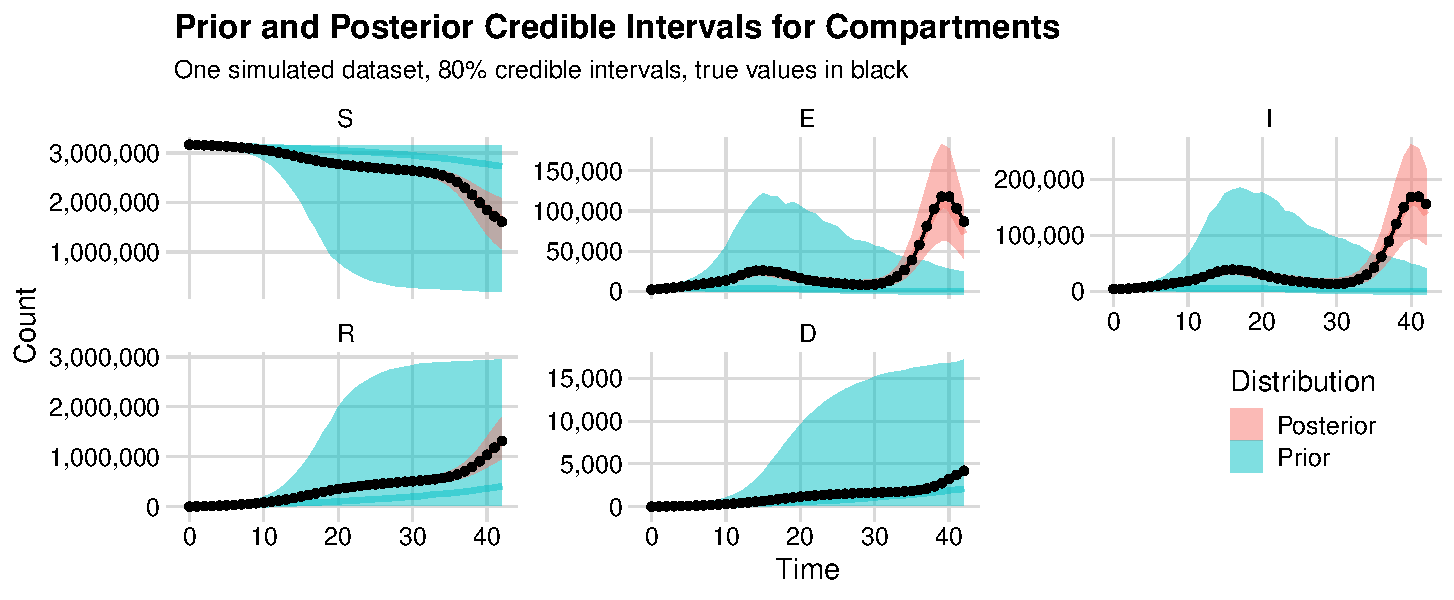
\includegraphics[width=1.0\columnwidth]{single_generated_quantities_simulation_compartment_plot}
    \caption{Prior and posterior 80\% credible intervals for latent compartments for a model fit to the dataset presented in Figure~\ref{ch_4:fig:simulated_binned_data_plot}.
    True values for the simulated compartment sizes are indicated by solid black lines.}
    \label{ch_4:fig:single_generated_quantities_simulation_compartment_plot}
\end{figure}

\begin{figure}[htbp]
    \centering
    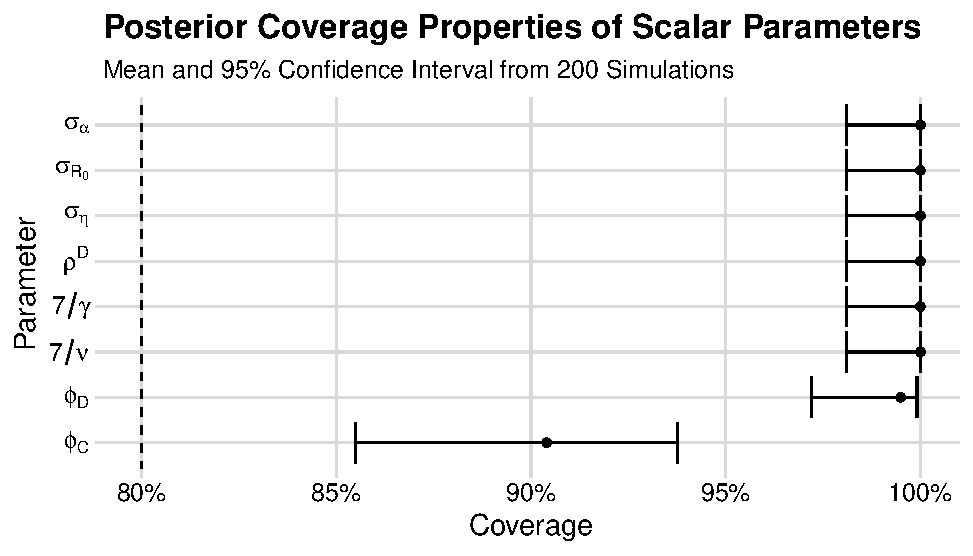
\includegraphics[width=1.0\columnwidth]{generated_quantities_simulation_scalar_coverage_plot}
    \caption{Coverage properties of 80\% posterior credible intervals for scalar parameters from models fit to 200 simulated datasets.
    Nominal coverage is indicated by the dashed line.}
    \label{ch_4:fig:generated_quantities_simulation_scalar_coverage_plot}
\end{figure}

\begin{figure}[htbp]
    \centering
    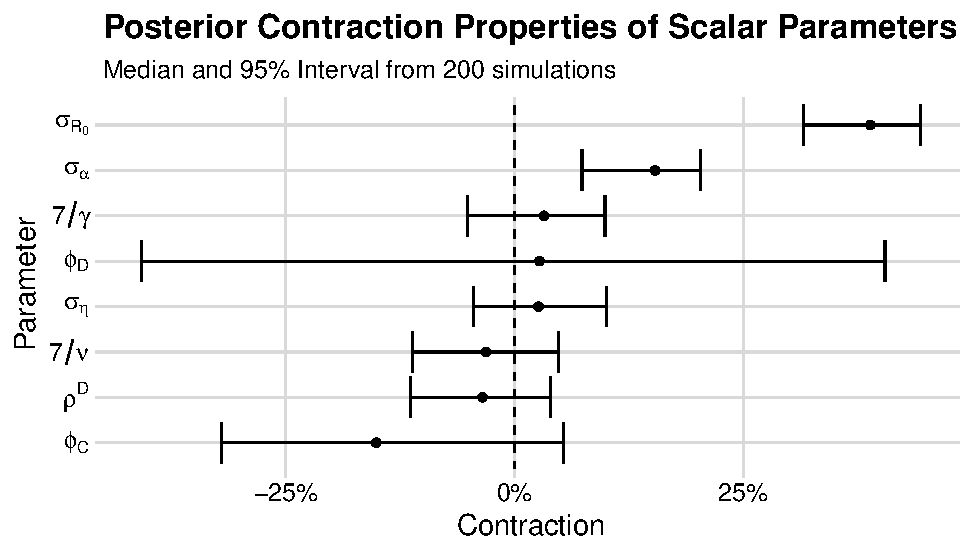
\includegraphics[width=1.0\columnwidth]{generated_quantities_simulation_scalar_shrinkage_plot}
    \caption{Contraction properties of scalar parameters from models fit to 200 simulated datasets.
    Contraction is calculated as one minus the ratio of standard deviation of the posterior and the prior.}
    \label{ch_4:fig:generated_quantities_simulation_scalar_shrinkage_plot}
\end{figure}

\begin{figure}[htbp]
    \centering
    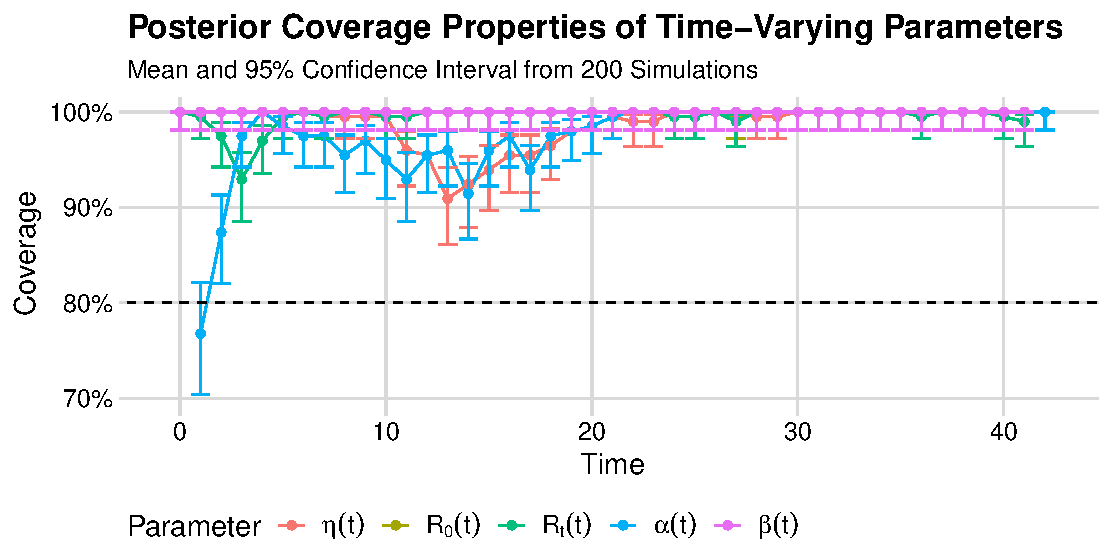
\includegraphics[width=1.0\columnwidth]{generated_quantities_simulation_time_varying_coverage_plot}
    \caption{Coverage properties of 80\% posterior credible intervals for time-varying parameters from models fit to 200 simulated datasets.
    Nominal coverage is indicated by the dashed line.}
    \label{ch_4:fig:generated_quantities_simulation_time_varying_coverage_plot}
\end{figure}

\begin{figure}[htbp]
    \centering
    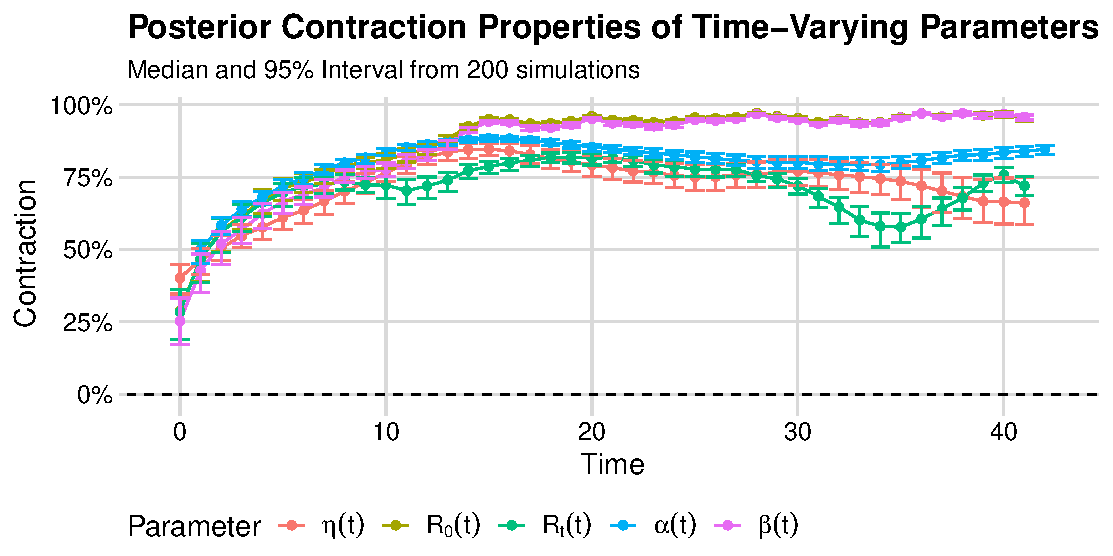
\includegraphics[width=1.0\columnwidth]{generated_quantities_simulation_time_varying_shrinkage_plot}
    \caption{Contraction properties of time-varying parameters from models fit to 200 simulated datasets.
    Contraction is calculated as one minus the ratio of standard deviation of the posterior and the prior.}
    \label{ch_4:fig:generated_quantities_simulation_time_varying_shrinkage_plot}
\end{figure}

\begin{figure}[htbp]
    \centering
    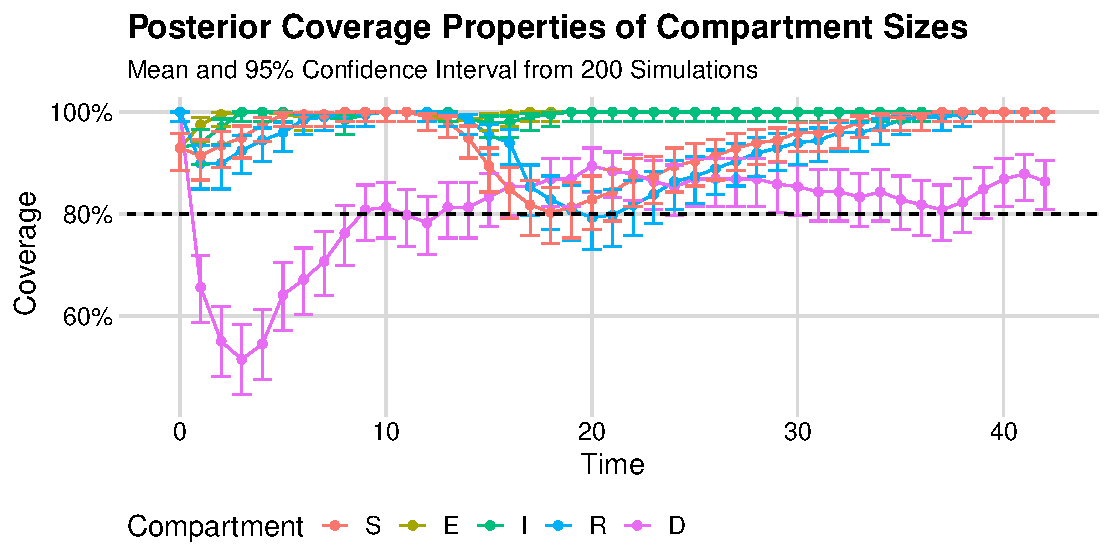
\includegraphics[width=1.0\columnwidth]{generated_quantities_simulation_compartment_coverage_plot}
    \caption{Coverage properties of 80\% posterior credible intervals for latent compartments from models fit to 200 simulated datasets.
    Nominal coverage is indicated by the dashed line.}
    \label{ch_4:fig:generated_quantities_simulation_compartment_coverage_plot}
\end{figure}

\begin{figure}[htbp]
    \centering
    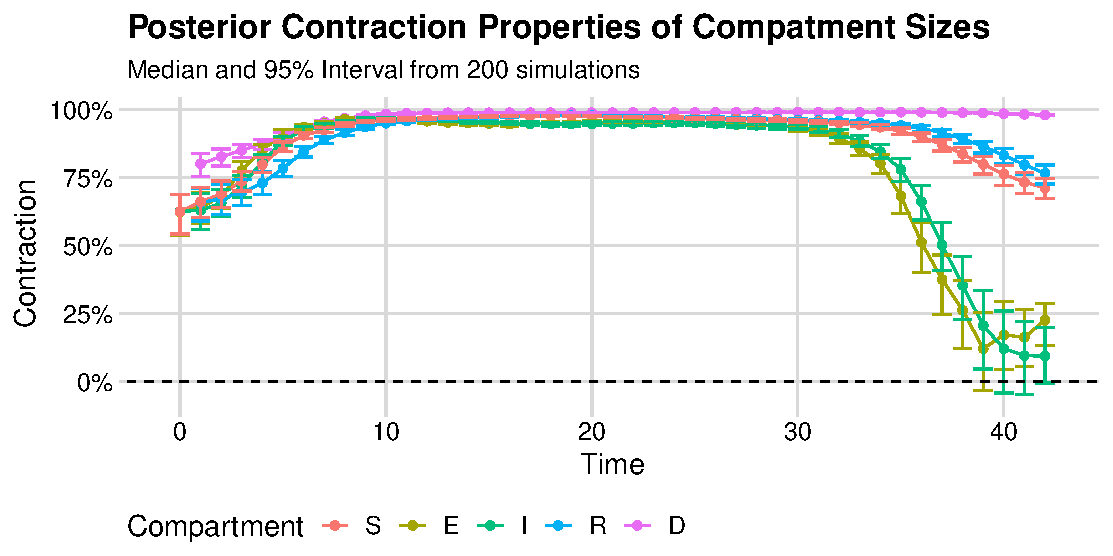
\includegraphics[width=1.0\columnwidth]{generated_quantities_simulation_compartment_shrinkage_plot}
    \caption{Contraction properties of latent compartments from models fit to 200 simulated datasets.
    Contraction is calculated as one minus the ratio of standard deviation of the posterior and the prior.}
    \label{ch_4:fig:generated_quantities_simulation_compartment_shrinkage_plot}
\end{figure}

\section{Comparison with \texttt{epidemia}}
\label{ch_4:epidemia_section}

We used the \texttt{epidemia} R package to infer \( R_t \) in the same 200 simulated datasets, as well as the Orange County data. 
Statistical details of these methods are presented below.
Commentary on these results is presented in Section~\ref{ch_4:sec:results} of the main text.

The \texttt{epidemia} package can be used to create different branching process inspired models to estimate the effective reproduction number. In contrast to the compartmental model used in this paper, branching process inspired models have related the mean of current incidence to a weighted sum of previous incidence and the effective reproduction number $R_{t}$. Let $I_{t}$ be the incidence at time $t$, $R_{t}$ be the effective reproduction number at time $t$, and $g(t)$ be the probability density function of the generation time distribution (the time between an individual becoming infected and infecting another individual; under the compartmental model framework this is usually taken to be equivalent to the sum of the latent period and the infectious period). Then the mean relationship used is:
\begin{equation*}
    E[I_{t}|I_{1}, \dots, I_{t-1}] = R_{t}\sum_{s=1}^{t-1}I_{s}g(t-s).
\end{equation*}
For the model we used in this study, we then added an observation model for new cases, modeled the effective reproduction number as a random walk, and modeled unobserved incidence as an autoregressive normal random variable with variance equal to the mean multiplied by an over-dispersion parameter.
 \begin{align*}
\tau &\sim \text{exp}(\lambda)  \quad \quad \text{Hyperprior for unobserved incidence}\\
I_{\nu} &\sim \text{exp}(\tau) \quad \quad \text{Prior on unobserved incidence $\nu$ days before observation}\\
I_{\nu+1}, \dots, I_{0} &= I_{\nu}  \quad \quad \text{Unobserved incidence}\\
    \sigma & \sim \text{Truncated-Normal}(0, 0.1^{2}) \\
   \log{R_{0}} &\sim \text{Normal}(\log{2}, 0.2^{2})\quad \quad \text{Prior on $R_{0}$} \\
    \log{R_{t}}|\log{R_{t-1}} &\sim \text{Normal}(\log{R_{t-1}}, \sigma)  \quad \quad \text{Random Walk prior on $R_{t}$}\\
\psi &\sim \text{Normal}(10,2) \quad \quad \text{Prior on variance parameter for incidence} \\
I_{t}|I_{\nu}, \dots, I_{t-1} &\sim \text{Normal}(R_{t}\sum_{s<t}I_{s}g_{t-s}, \psi) \quad \quad \text{Model for incidence} \\
    \alpha &\sim \text{Normal}(0.13, 0.7^2)
\quad \quad \text{Prior on case detection rate} \\
y_{t} &= \alpha_{t}\sum_{s<t}I_{s}\pi_{t-s} \quad \quad \text{Mean of observed data model}\\
\phi & \sim P(\phi) \quad \quad \text{Prior on dispersion parameter for observed data} \\
Y_{t} &\sim \text{Neg-Binom}(y_{t}, \phi) \quad \quad \text{Observed data model}\\
\end{align*}
Here $\pi_{t}$ are the values of the probability density function for the delay distribution, the time between an individual being infected and being observed.
This distribution is assumed to be a gamma distribution with shape parameter one and mean equal to the true mean latent period. 
To sample from the posterior distribution, \texttt{epidemia} uses Hamiltonian Monte Carlo via the \texttt{Stan} simulation software \citep{rstan}.
We draw 2000 posterior samples and discard the first 1000 for this analysis.


\begin{figure}[htbp]
    \centering
    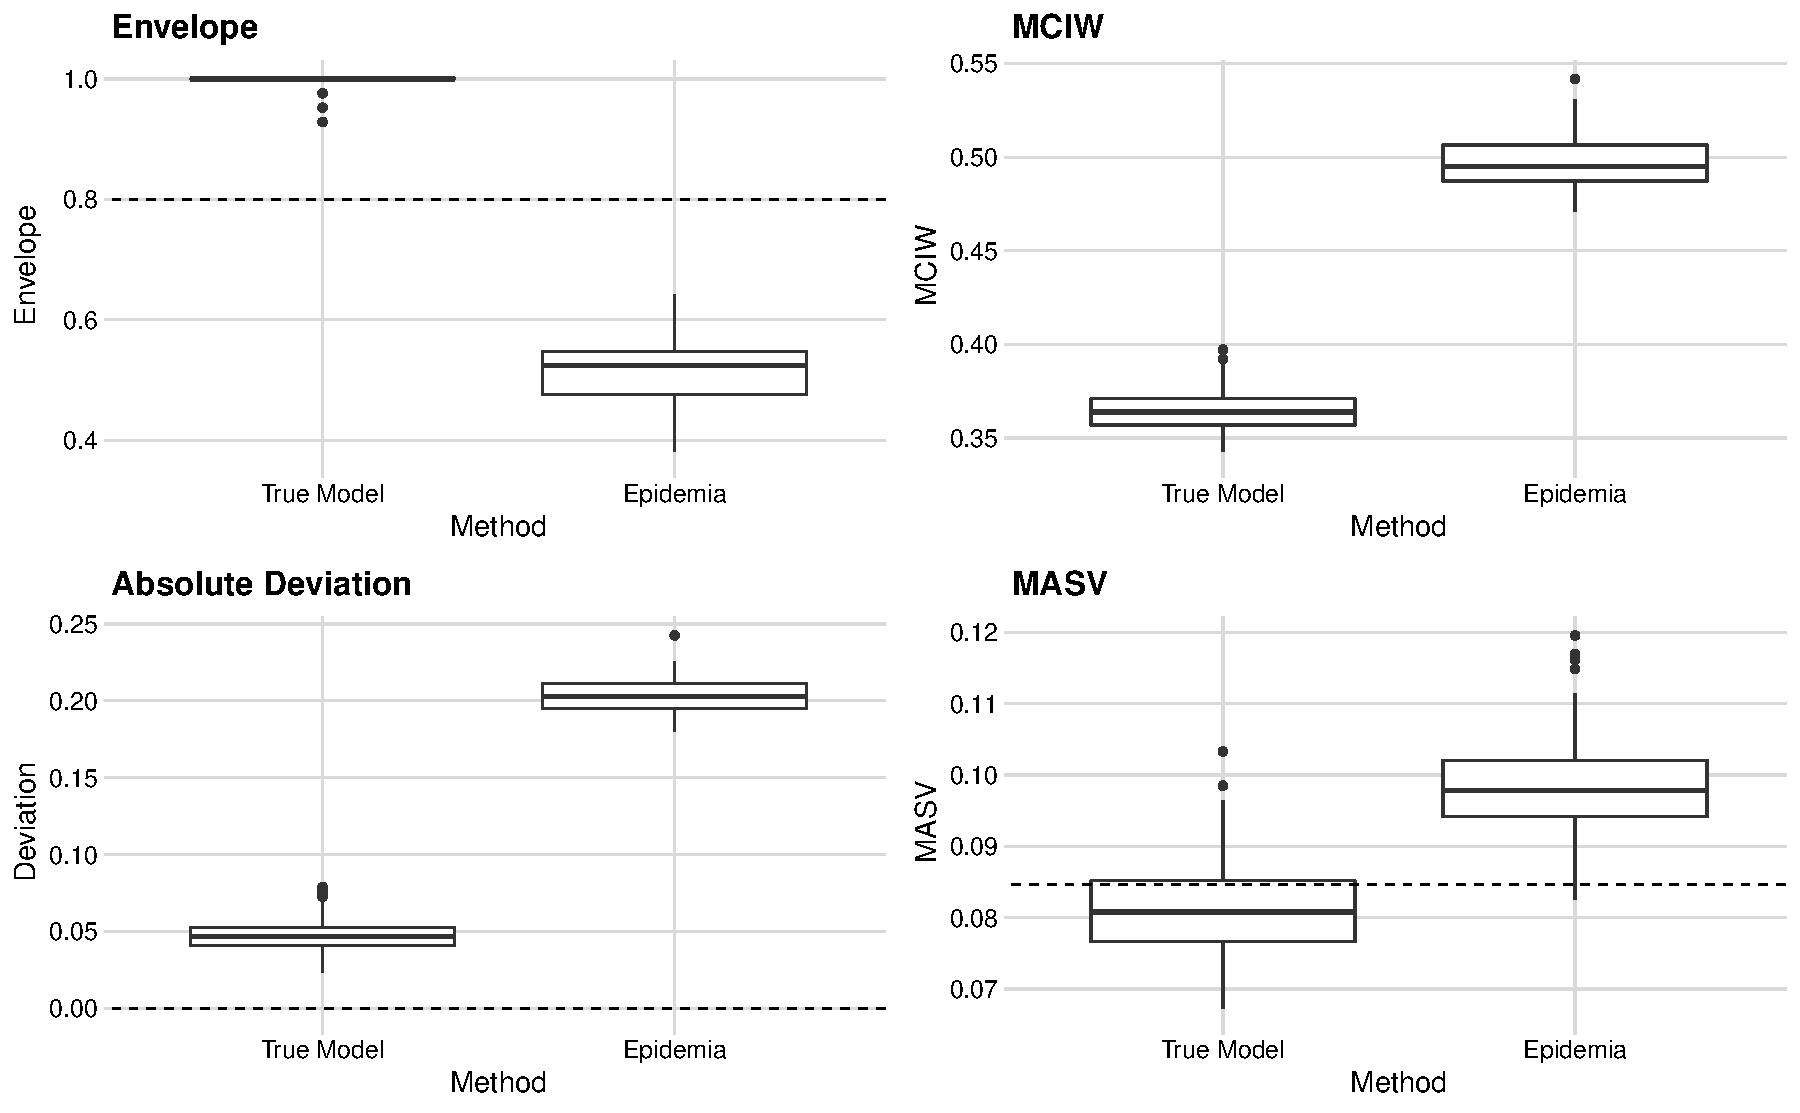
\includegraphics[width=1.0\columnwidth]{rt_comparison_metrics_plot}
    \caption{Properties of \( R_t \) estimation from 200 simulated data sets.
    The envelope is the proportion of time points which the 80\% posterior credible interval contains the true \( R_t \) value specified in the simulation.
    Mean credible interval width (MCIW) is the mean of credible interval widths across time points within a simulation replication.
    Absolute deviation is calculated as the mean of the absolute difference between the posterior median and the true \( R_t \) value at each time point.
    The mean absolute sequential variation (MASV) is the mean of the absolute difference between the posterior median at a time point and the posterior median at the previous time point.}
    \label{ch_4:fig:rt_comparison_metrics_plot}
\end{figure}

\section{Comparison with modeling structured populations}
\label{ch_4:sec:hetero}
Here, we demonstrate that semi-parametric modeling of key parameters can obviate the need for modeling heterogeneous populations with separate compartments.
We construct a model wherein a disease spreads among two subpopulations: the ``general" population and the ``vulnerable" population, which interact with each other.
Progression through compartments is governed by the following system of differential equations, with ``g" subscripts denoting the general subpopulation and ``v" subscripts denoting the vulnerable subpopulation and parameters having the same interpretations as in the main text.
The differential equations used for this model presented in \eqref{eqn:model_hetero_SIR_ODEs}.

\begin{equation}
\label{ch_4:eqn:model_hetero_SIR_ODEs}
\begin{aligned}
\deriv{S_v}{t} &= -\left(\beta_{vv} I_v + \beta_{vg} I_g \right) \frac{S_v}{N} \\
\deriv{E_v}{t} &= \left(\beta_{vv} I_v + \beta_{vg} I_g \right) \frac{S_v}{N} - \gamma E_v \\
\deriv{I_v}{t} &= \gamma E_v - \nu I_v \\
\deriv{R_v}{t} &= \nu (1-\eta_v) I_v \\
\deriv{D_v}{t} &= \nu \eta_v I_v \\
\end{aligned}
\qquad \qquad \qquad
\begin{aligned}
\deriv{S_g}{t} &= -\left(\beta_{gg} I_g + \beta_{gv} I_v\right) \frac{S_g}{N} \\
\deriv{E_g}{t} &= \left(\beta_{gg} I_g + \beta_{gv} I_v \right) \frac{S_g}{N} - \gamma E_g \\
\deriv{I_g}{t} &= \gamma E_g - \nu I_g \\
\deriv{R_g}{t} &= \nu (1-\eta_g) I_g \\
\deriv{D_g}{t} &= \nu \eta_g I_g \\
\end{aligned}
\end{equation}

subject to initial conditions $ \bX(t_0) = \bx_0 $ and $ \bN(t_0) = \mathbf{0}$, where $\bx_0 = (S_{v0}, E_{v0}, I_{v0}, R_{v0}, \linebreak[0] D_{v0}, S_{g0}, E_{g0}, I_{g0}, R_{g0}, D_{g0})$ are initial compartment counts.

We only observed the unstratified case and death counts.
Observed cases and deaths are Poisson distributed with the rate parameter equal to the number of latent cases and deaths, respectively.

\[ Y_l \sim \text{Poisson}(\Delta N_{E_v I_v}(t_l) + \Delta N_{E_g I_g}(t_l)) \]
\[ M_l \sim \text{Poisson}(\Delta N_{I_v D_v}(t_l) + \Delta N_{I_g D_g}(t_l)) \]

We construct a scenario where a disease outbreak occurs in a small vulnerable population with a true infection-fatality ratio of 10\% before spreading to a larger general population with a true infection-fatality ratio of 1\%.
Because the outbreak spreads through the different populations at different times, the true population infection-fatality ratio varies in time.
Figure~\ref{ch_4:fig:data_ifr_age_structure_plot} shows the latent new cases and new deaths for each subpopulation, as well as the combined latent new cases and new deaths, and the observed new cases and new deaths for this constructed scenario.

\begin{figure}[htbp]
    \centering
    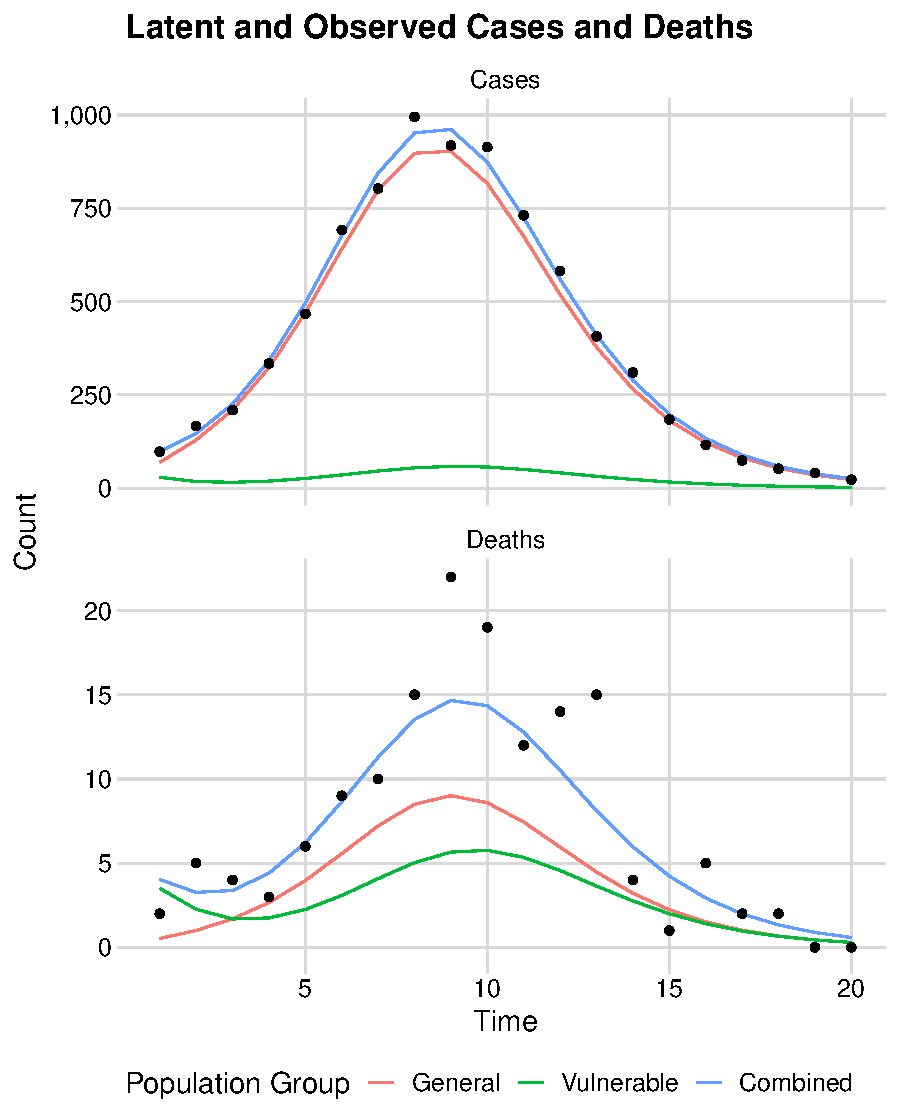
\includegraphics[width=0.75\columnwidth]{data_ifr_age_structure_plot}
    \caption{Latent new cases and deaths for vulnerable and general subpopulations, along with combined latent new cases and new deaths and observed (combined) new cases and new deaths for a simulated scenario.}
    \label{ch_4:fig:data_ifr_age_structure_plot}
\end{figure}

Now, we fit a semi-parametric model, similar to the one in the main text, to this data.
We model \( \eta(t) \) with a logit-Guassian Markov random field, as in the main text.
The differential equations used for this model presented in \eqref{eqn:model_nonparametric_SIR_ODEs}.
\begin{equation}
\label{ch_4:eqn:model_nonparametric_SIR_ODEs}
\begin{aligned}
\deriv{S}{t} &= - \beta I \frac{S}{N}\\
\deriv{E}{t} &= \beta I \frac{S}{N} - \gamma E\\
\deriv{I}{t} &= \gamma E - \nu I\\
\deriv{R}{t} &= \nu (1 - \eta(t)) I\\
\deriv{D}{t} &= \nu \eta(t) I\\
\end{aligned}
\end{equation}

subject to initial conditions $ \bX(t_0) = \bx_0 $ and $ \bN(t_0) = \mathbf{0}$, where $\bx_0 = (S_0, E_0, I_0, R_0, D_0)$ are initial compartment counts.

Figures~\ref{ch_4:fig:posterior_predictive_ifr_age_structure_plot}--\ref{ch_4:fig:ifr_age_structure_generated_quantities_simulation_time_varying_plot}, demonstrate, that when we fit our semi-parametric model, we can generally fit the data well and recover the true values of the parameters without modeling the two heterogeneous populations.

\begin{figure}[htbp]
    \centering
    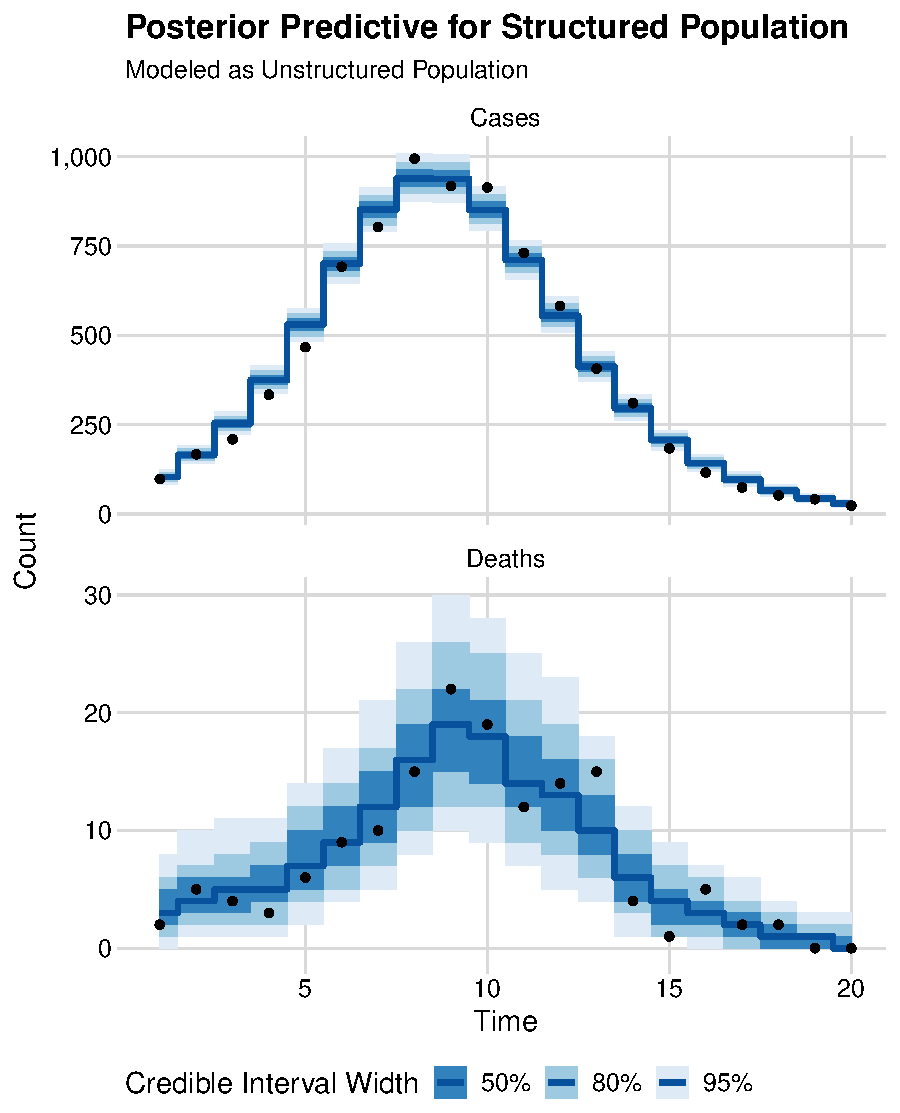
\includegraphics[width=0.75\columnwidth]{posterior_predictive_ifr_age_structure_plot}
    \caption{Posterior predictive distributions for a model with non-parametric IFR fit to a simulated dataset with a heterogeneous population.
    The case and death data used are shown as black dots.}
    \label{ch_4:fig:posterior_predictive_ifr_age_structure_plot}
\end{figure}

\begin{figure}[htbp]
    \centering
    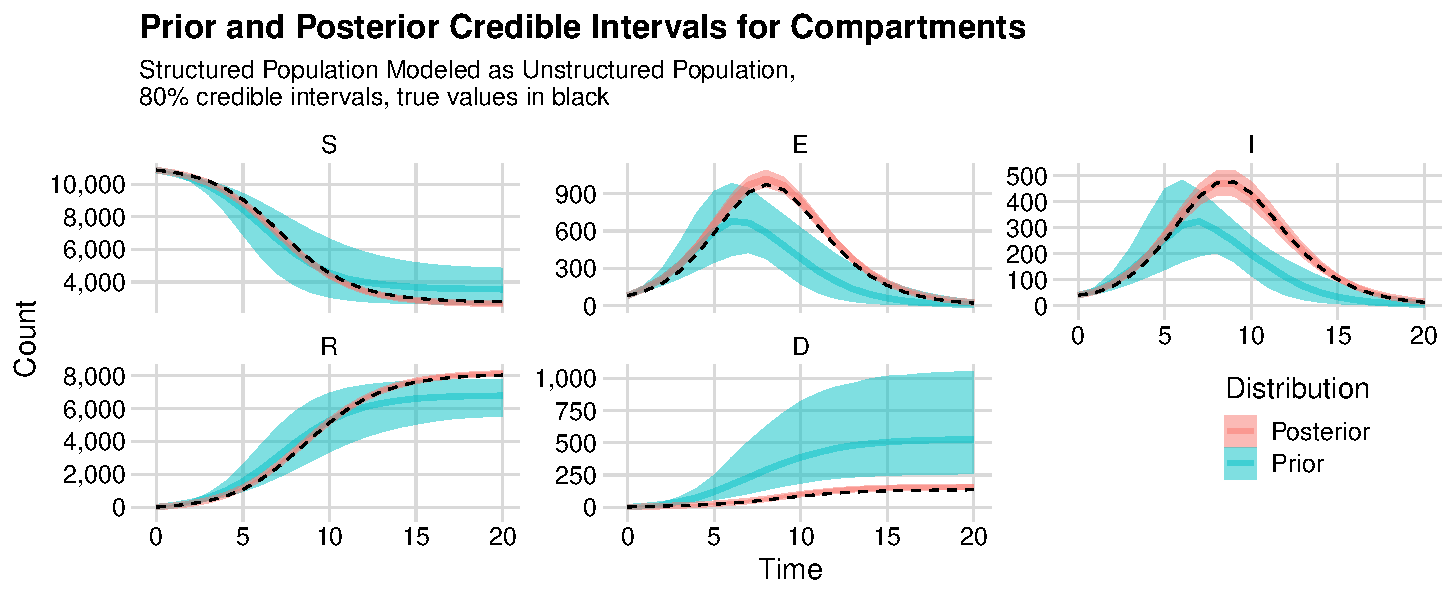
\includegraphics[width=0.75\columnwidth]{ifr_age_structure_generated_quantities_simulation_compartment_plot}
    \caption{Prior and Posterior distributions for latent compartments for a model with non-parametric IFR fit to a simulated dataset with a heterogeneous population.
    The true time-varying parameters are indicated by the dashed line.}
    \label{ch_4:fig:ifr_age_structure_generated_quantities_simulation_compartment_plot}
\end{figure}


\begin{figure}[htbp]
    \centering
    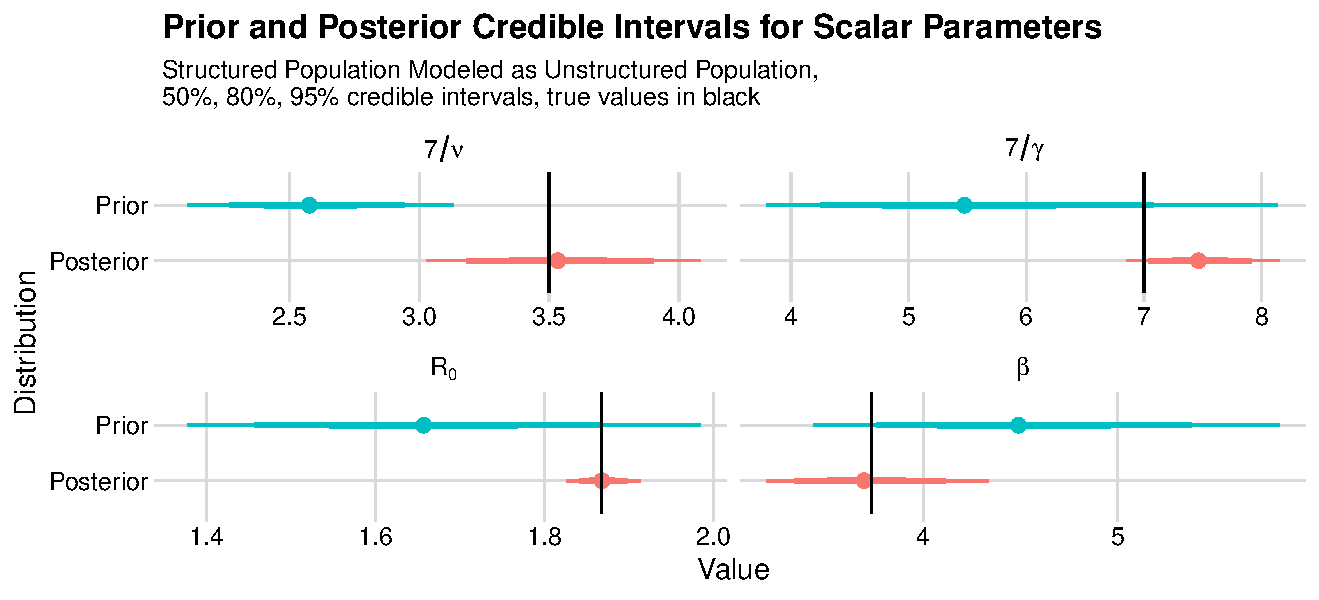
\includegraphics[width=0.75\columnwidth]{ifr_age_structure_generated_quantities_simulation_scalar_plot}
    \caption{Prior and posterior distributions for scalar parameters for a model with non-parametric IFR fit to a simulated dataset with a heterogeneous population.
    The true time-varying parameters are indicated by the vertical line.}
    \label{ch_4:fig:ifr_age_structure_generated_quantities_simulation_scalar_plot}
\end{figure}

\begin{figure}[htbp]
    \centering
    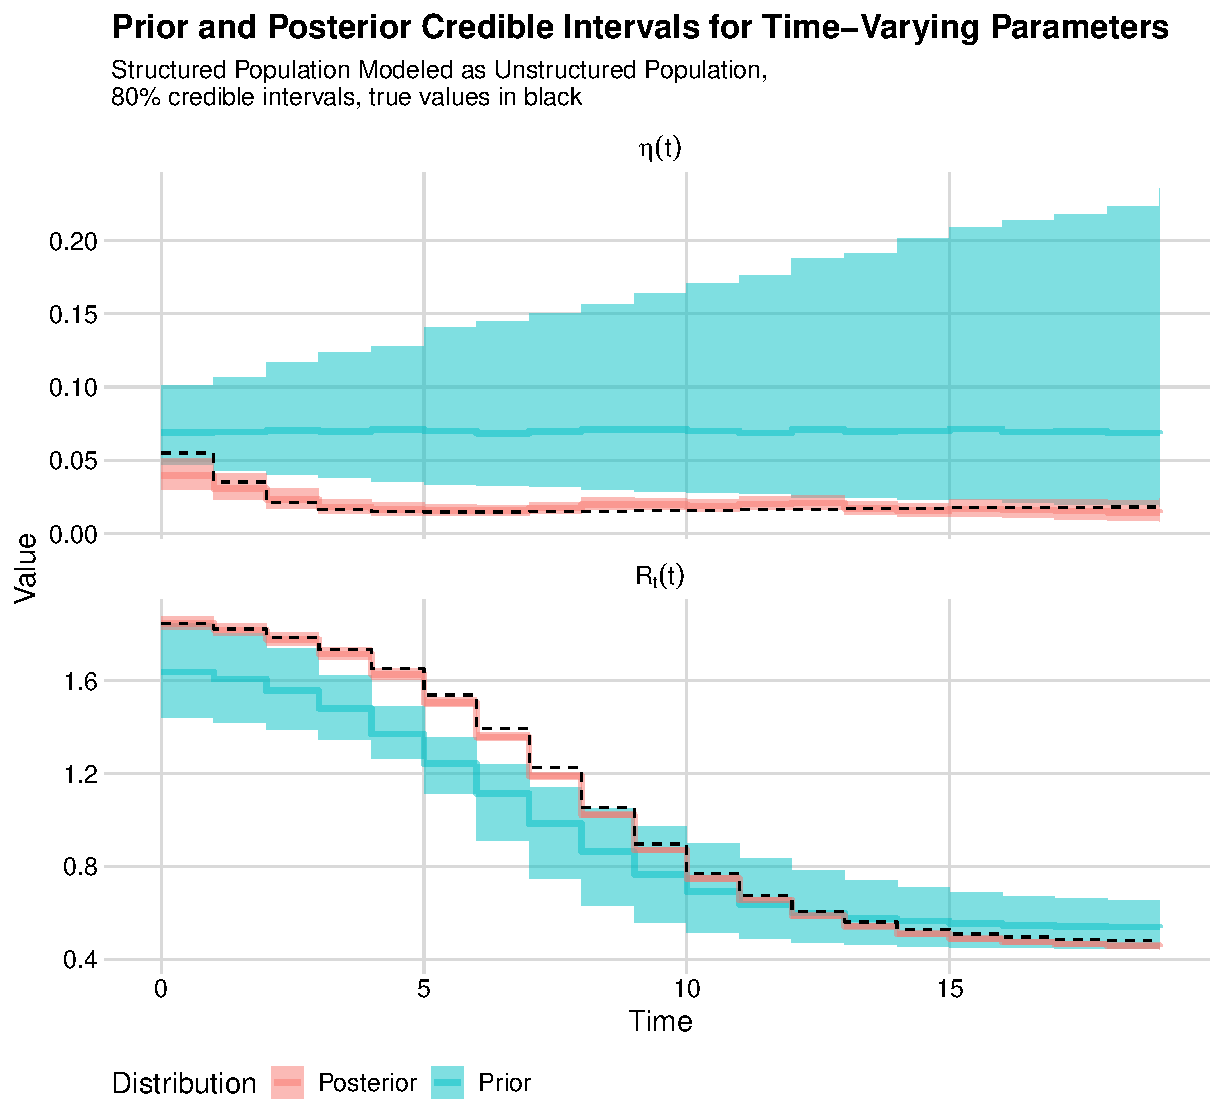
\includegraphics[width=0.75\columnwidth]{ifr_age_structure_generated_quantities_simulation_time_varying_plot}
    \caption{Prior and Posterior distributions for time-varying parameters for a model with non-parametric IFR fit to a simulated dataset with a heterogeneous population.
    The true time-varying parameters are indicated by the dashed line.}
    \label{ch_4:fig:ifr_age_structure_generated_quantities_simulation_time_varying_plot}
\end{figure}

\section{Sensitivity analysis}
\label{ch_4:sec:sensitivity}
We conducted four sensitivity analyses to see how our results change depending on the specified priors.
In each additional analysis, we change only one aspect of the model priors.
We perform one analysis where, \textit{a priori}, twice the number of people are initially infected (denoted Half \( S_0 \)), one with a lower initial basic reproduction number prior (denoted Half \( \exp\left( \tilde{R} _{0,1} \right) \), one with a higher initial infection fatality ratio prior (denoted Double \( \expit \left( \tilde{\eta}_1 \right) \), and one with a lower initial $\alpha$ prior (denoted Half \( \exp \left( \tilde{\alpha}_1 \right) \).
Precise descriptions of the priors used in the sensitivity analyses are presented in Table~\ref{ch_4:table:sensitivity_priors}.
Graphical results of the sensitivity analyses are presented in Figures~\ref{ch_4:fig:scalar_sensitivity_plot}--\ref{ch_4:fig:compartments_sensitivity_plot}.
We find that our model is typically robust to these alternative priors, and no alternative model leads to substantively different conclusions.

% \begin{table}
%     \caption[Sensitivity analysis priors.]{Model parameters and their prior distributions.}
%     \label{ch_4:table:sensitivity_priors}
%     \scriptsize\centering
%     \begin{tabularx}{\columnwidth}{cclclc}
% 	\thead{Analysis} & \thead{Parameter} & \thead{Original Prior}  &   \thead{Original Prior\\Median\\(95\% Interval)}  &   \thead{Sensitivity Prior} &   \thead{Sensitivity Prior\\Median\\(95\% Interval)}    \\ \hline
%     Half \( S_0 \)  &   \( S_0 \)   &   Logit-Normal(6, 0.25) & \makecell{0.998 \\ (0.993, 0.999)}  &   Logit-Normal(5.31, 0.25) & \makecell{0.995 \\ (0.987, 0.998)}  \\
%     Half \( \exp\left( \tilde{R} _{0,1} \right) \)  &   \( \exp\left( \tilde{R} _{0,1} \right) \)   &   Log-Normal(0, 0.0625) & \makecell{1.000 \\ (0.613, 1.630)} &   Log-Normal(-0.693, 0.0625) & \makecell{0.500 \\ (0.306, 0.816)} \\
%     Double \( \expit \left( \tilde{\eta}_1 \right) \)  &    \( \expit \left( \tilde{\eta}_1 \right) \)  &   Logit-Normal(-5.3, 0.04) & \makecell{0.00497 \\ (0.00336, 0.00733)}  &   Logit-Normal(-4.61, 0.04) & \makecell{0.00988 \\ (0.00670, 0.01460)} \\
%     Half \( \exp \left( \tilde{\alpha}_1 \right) \)  &  Half \( \exp \left( \tilde{\alpha}_1 \right) \) &   Log-Normal(1.35, 0.0121) & \makecell{3.86 \\ (3.11, 4.79)}  &   Log-Normal(0.657, 0.0121) & \makecell{1.93 \\ (1.55, 2.39)} \\
%     \end{tabularx}
% \end{table}


\begin{table}
    \caption[Sensitivity analysis priors.]{Model parameters and their prior distributions.}
    \label{ch_4:table:sensitivity_priors}
    \centering
    \begin{tabular}{llcc}
	\thead{Analysis}   &   \thead{Parameter}   &   \thead{Original Prior\\Median\\(95\% Interval)} &   \thead{Sensitivity Prior\\Median\\(95\% Interval)}  \\ \hline
    Half \( S_0 \)  &   \( S_0 \)   &   \makecell{0.998 \\ (0.993, 0.999)}  &   \makecell{0.995 \\ (0.987, 0.998)}  \\
    Half \( \exp\left( \tilde{R} _{0,1} \right) \)  &   \( \exp\left( \tilde{R} _{0,1} \right) \)   &   \makecell{1.000 \\ (0.613, 1.630)}  &   \makecell{0.500 \\ (0.306, 0.816)} \\
    Double \( \expit \left( \tilde{\eta}_1 \right) \)   &   \( \expit \left( \tilde{\eta}_1 \right) \)  &   \makecell{0.00497 \\ (0.00336, 0.00733)}    &   \makecell{0.00988 \\ (0.00670, 0.01460)} \\
    Half \( \exp \left( \tilde{\alpha}_1 \right) \) &   Half \( \exp \left( \tilde{\alpha}_1 \right) \) &   \makecell{3.86 \\ (3.11, 4.79)} &   \makecell{1.93 \\ (1.55, 2.39)}
    \end{tabular}
\end{table}


\begin{figure}[htbp]
    \centering
    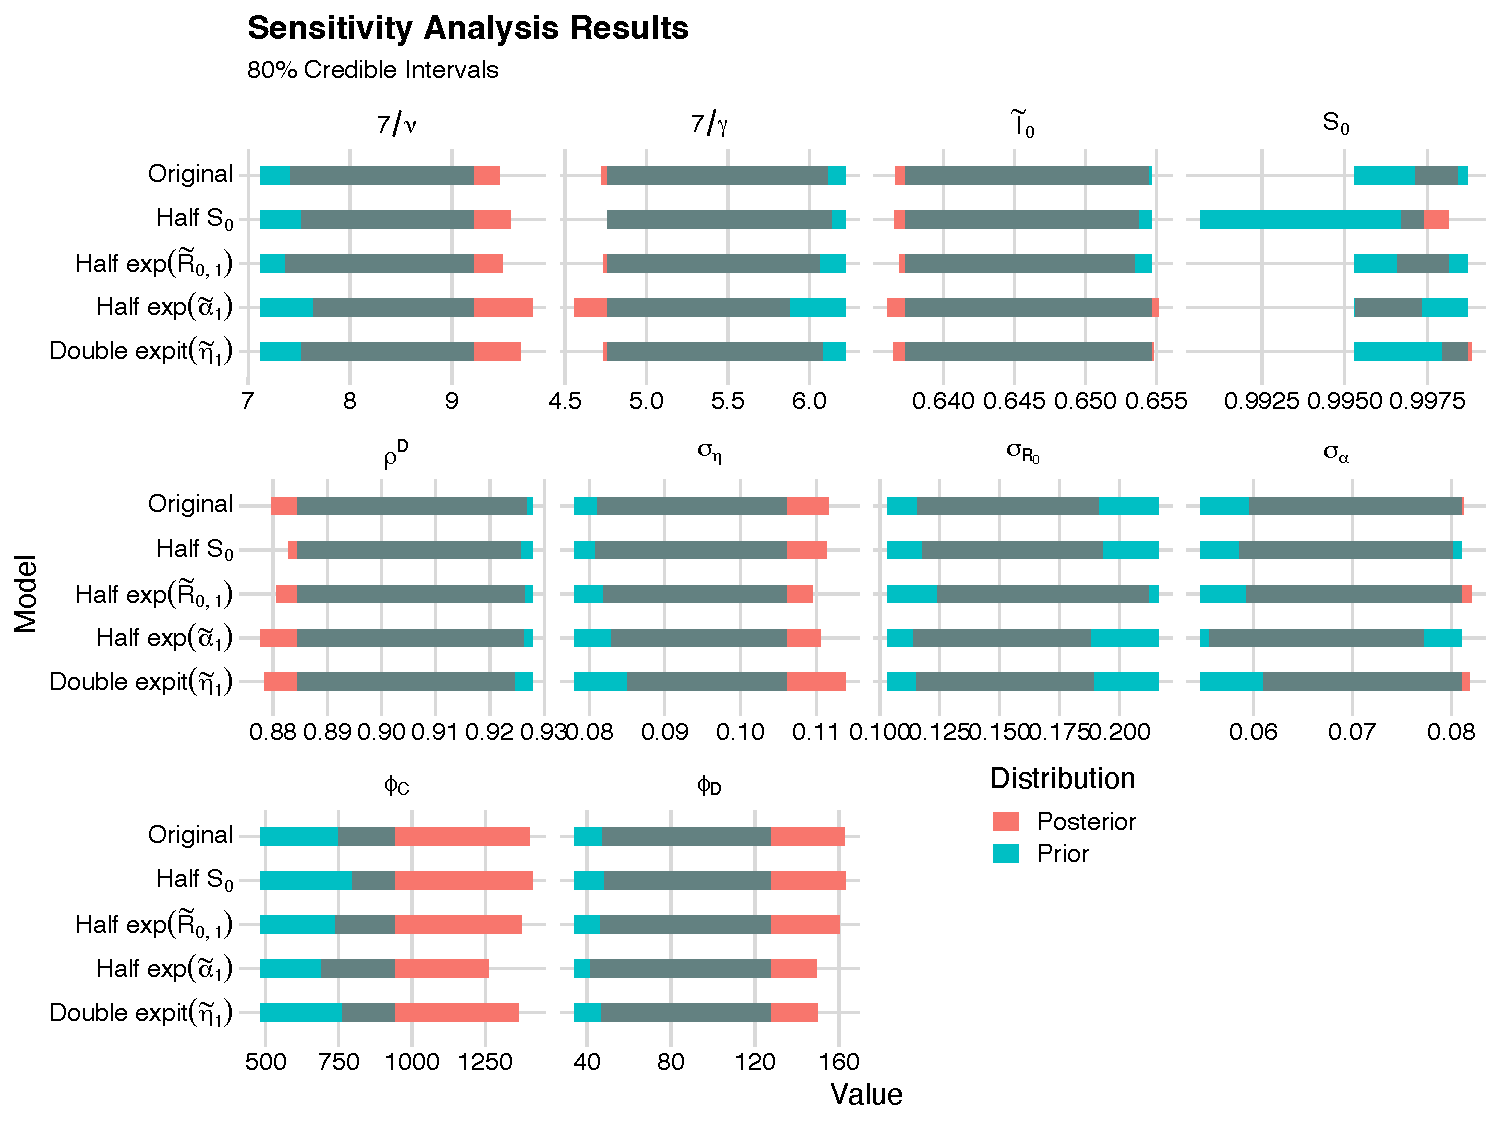
\includegraphics[width=1.0\columnwidth]{scalar_sensitivity_plot}
    \caption{
    Prior and posterior 80\% credible intervals for scalar parameters from four sensitivity analyses and the original analysis.}
    \label{ch_4:fig:scalar_sensitivity_plot}
\end{figure}

\begin{figure}[htbp]
    \centering
    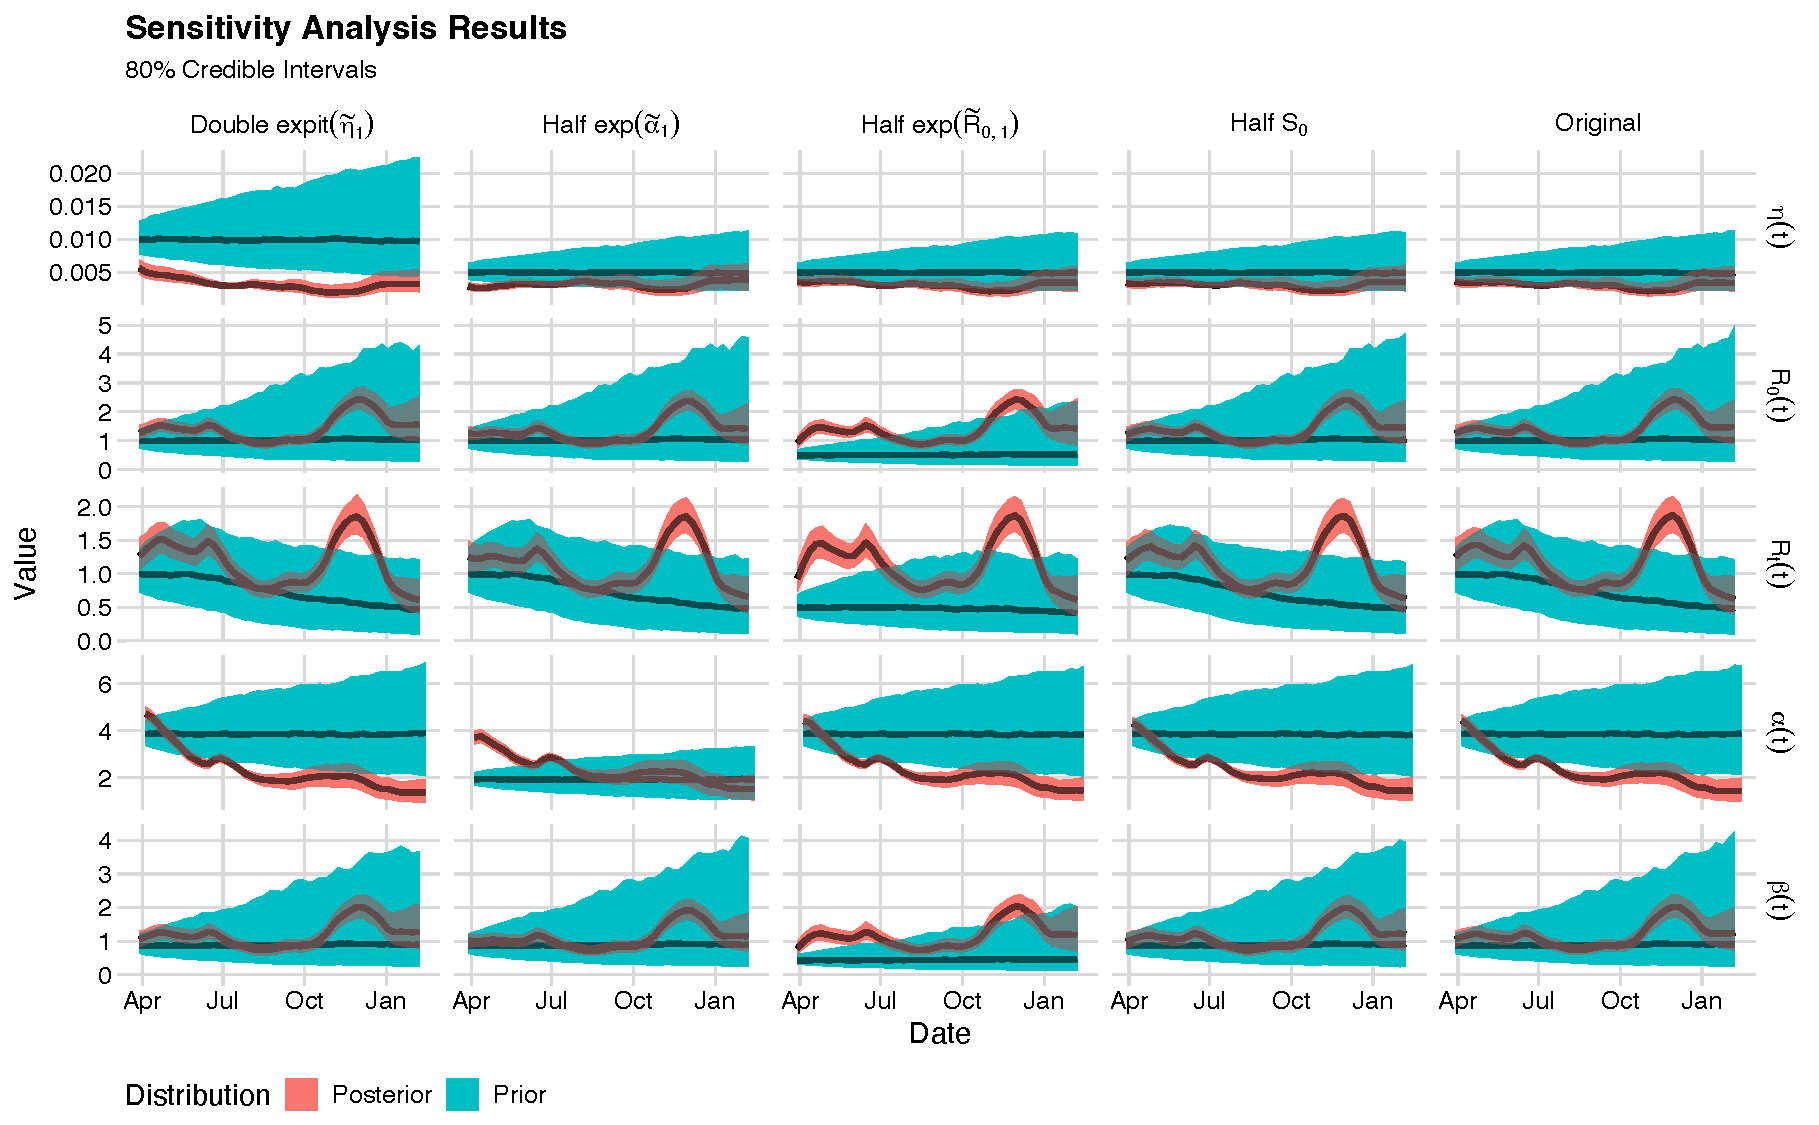
\includegraphics[width=1.0\columnwidth]{time_varying_sensitivity_plot}
    \caption{
    Prior and posterior 80\% credible intervals for time-varying parameters from four sensitivity analyses and the original analysis.}
    \label{ch_4:fig:time_varying_sensitivity_plot}
\end{figure}

\begin{figure}[htbp]
    \centering
    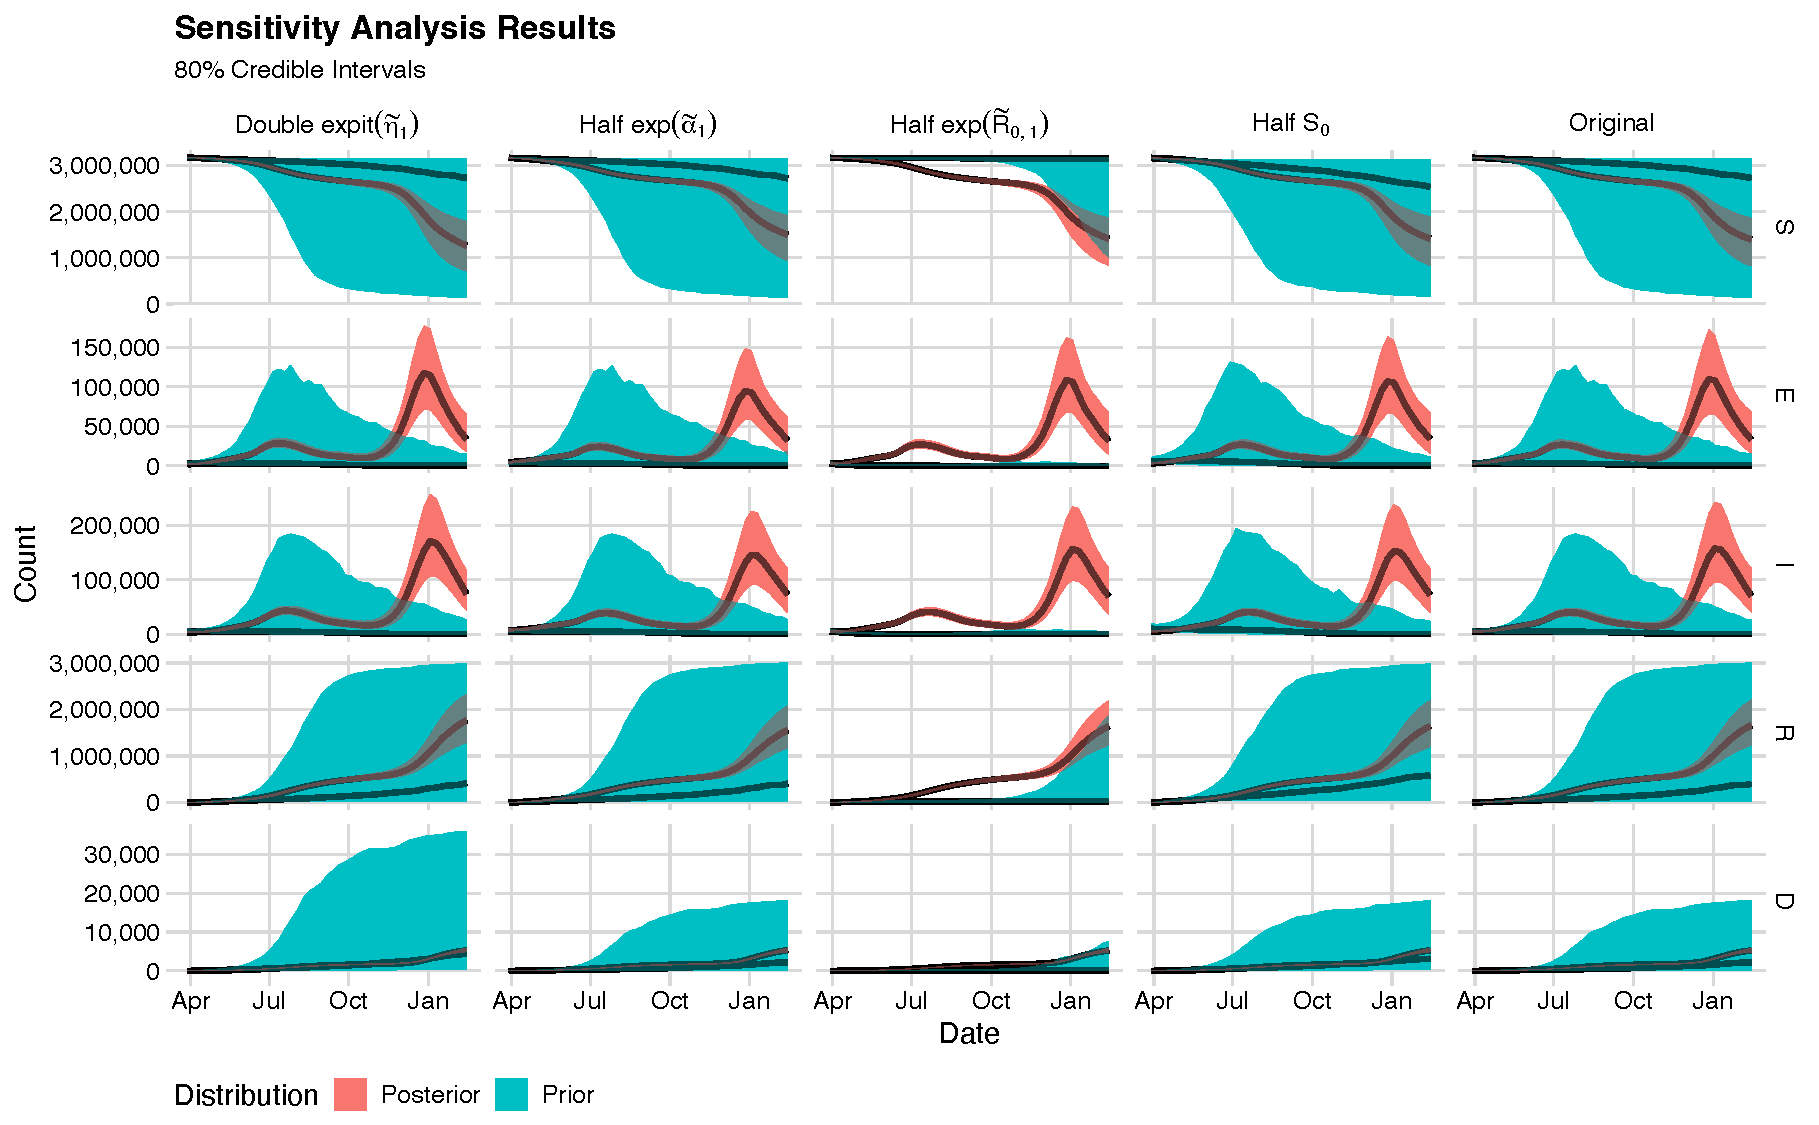
\includegraphics[width=1.0\columnwidth]{compartments_sensitivity_plot}
    \caption{Prior and posterior 80\% credible intervals for time-varying parameters from four sensitivity analyses and the original analysis.}
    \label{ch_4:fig:compartments_sensitivity_plot}
\end{figure}

Additionally, we perform analyses where we modify the main model to, one at a time, fix each of the time-varying parameters, \( R_0 \), \( \alpha \), and \( \eta \).
As demonstrated in Figure~\ref{ch_4:fig:compare_constant_time_varying_posterior_predictive_plot}, fixing these parameters has no negative impact on the model's ability to properly fit the test positivity and death data, with each of the models exhibiting nearly identical posterior predictive distributions.
However, these modified models do lead to substantially different inferences about the time-varying parameters themselves.
This is shown in Figure~\ref{ch_4:fig:compare_constant_time_varying_inference_plot}, where it appears that when one parameter is fixed, the others can become more flexible to still precisely match the observed data.
The most dramatic effect is seen when fixing \( R_0 \), which leads to drastically different inferences about \( \eta \) and \( \alpha \).
In contrast, there appears to be little impact from fixing the infection-fatality ratio, \( \eta \) as constant through time.

\begin{figure}[htbp]
    \centering
    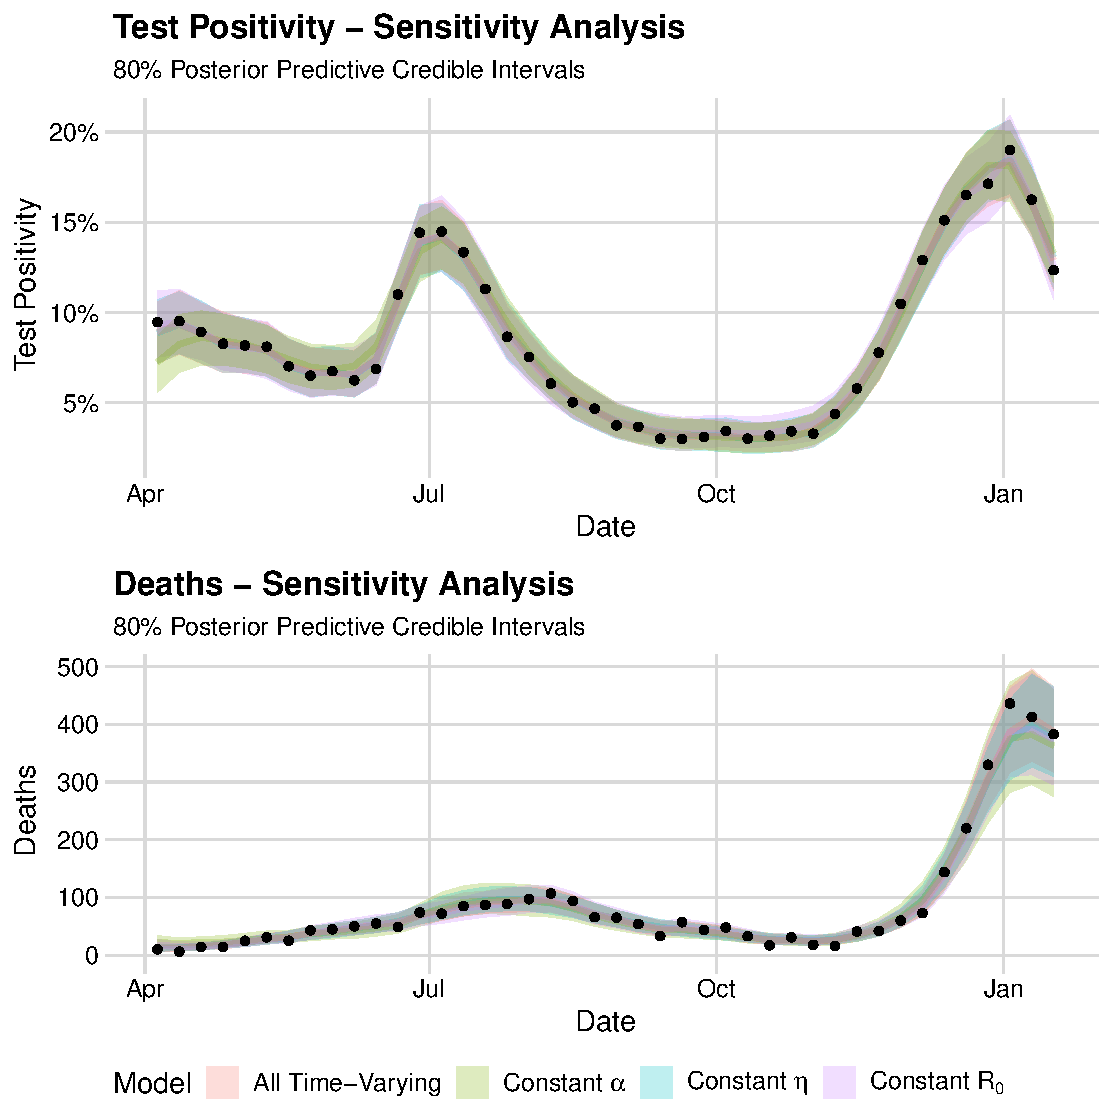
\includegraphics[width=1.0\columnwidth]{compare_constant_time_varying_posterior_predictive_plot}
    \caption{Posterior predictive distributions when one of the typically time-varying parameters is made to be fixed through time.}
    \label{ch_4:fig:compare_constant_time_varying_posterior_predictive_plot}
\end{figure}

\begin{figure}[htbp]
    \centering
    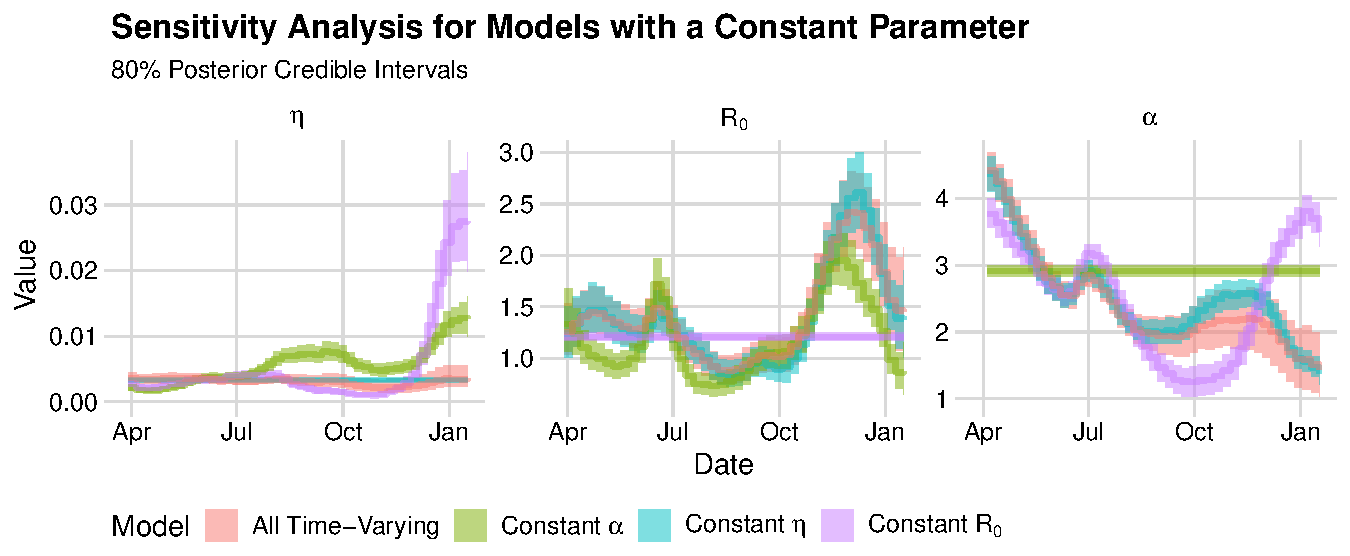
\includegraphics[width=1.0\columnwidth]{compare_constant_time_varying_inference_plot}
    \caption{Posterior inference for time-varying parameters when one of the typically time-varying parameters is made to be fixed through time.}
    \label{ch_4:fig:compare_constant_time_varying_inference_plot}
\end{figure}

\section{MCMC Diagnostics}
\label{ch_4:sec:convergence-diagnostics}

Convergence diagnostics are presented in Tables~\ref{ch_4:tab:univariate_diagnostics} and \ref{ch_4:tab:multivariate_diagnostics}, where $\hat{R}$ is the potential scale reduction factor \citep{Vehtari2021}, and ESS is the effective sample size, both as computed in the posterior R package \citep{posteriorPackage}.
All parameters show potential scale reduction factors between 1 and 1.02, providing no evidence of lack of convergence.
Additionally, all model parameters have effective sample sizes of multiple hundreds, which is sufficient for our inferences.

We also produce a trace plot of the log-posterior probability for each chain in Figure~\ref{ch_4:fig:lp_trace_plot}, which indicates that each chain explores a region of similar probability.

\input{tables/univariate_diagnostics}
\input{tables/multivariate_diagnostics}

\begin{figure}[htbp]
    \centering
    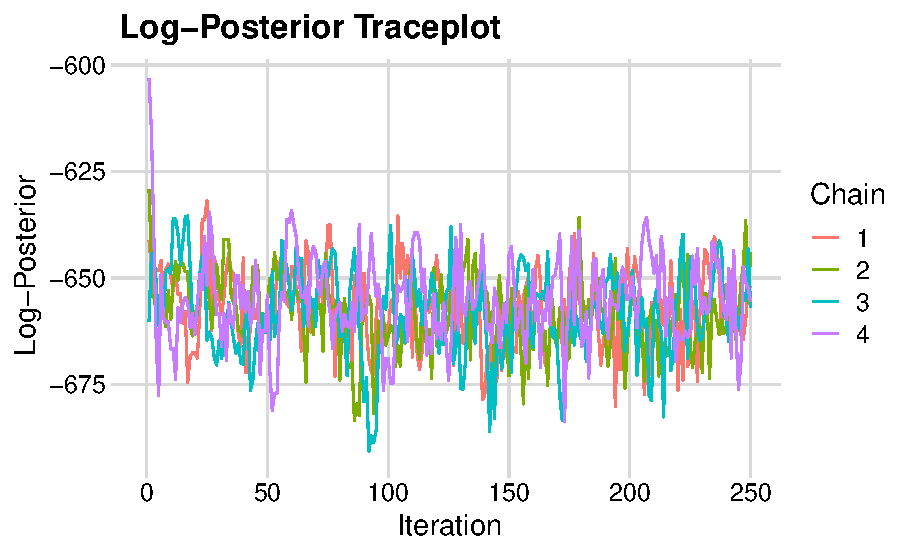
\includegraphics[width=1.0\columnwidth]{lp_trace_plot}
    \caption{Trace plot of log-posterior probability for the main model fit.}
    \label{ch_4:fig:lp_trace_plot}
\end{figure}

\addtocontents{toc}{\protect\setcounter{tocdepth}{2}}